\documentclass[tikz,border=8pt]{standalone}
\usepackage{amsmath,amssymb}
\usetikzlibrary{arrows.meta,automata,positioning,quotes}
\begin{document}
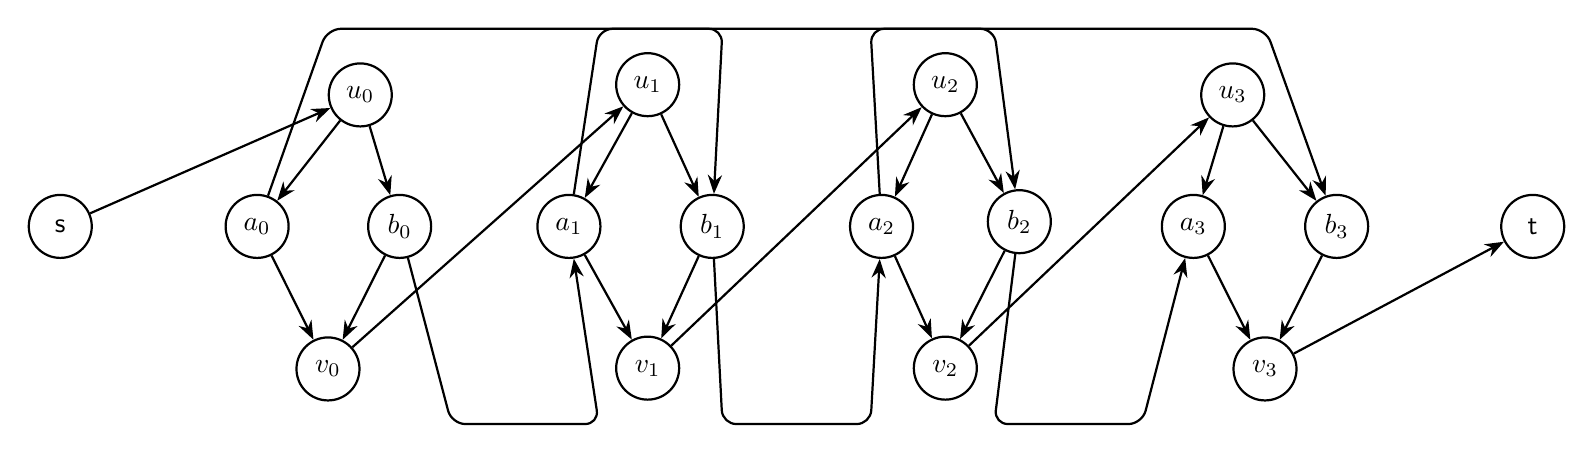
\begin{tikzpicture}[x=1cm,y=1cm]
\tikzset{
  graphnode/.style={circle,draw,thick,minimum size=8mm,inner sep=1pt,font=\sffamily},
  directed/.style={-{Stealth[length=2.4mm]},thick},
  undirected/.style={thick}
}
\node[graphnode] (n_s) at (-2.70,0.00) {s};
\node[graphnode] (n_u_0) at (1.11,1.67) {$u_{0}$};
\node[graphnode] (n_a_0) at (-0.20,0.00) {$a_{0}$};
\node[graphnode] (n_b_0) at (1.61,0.00) {$b_{0}$};
\node[graphnode] (n_v_0) at (0.70,-1.81) {$v_{0}$};
\node[graphnode] (n_u_1) at (4.76,1.80) {$u_{1}$};
\node[graphnode] (n_a_1) at (3.76,0.00) {$a_{1}$};
\node[graphnode] (n_b_1) at (5.58,0.00) {$b_{1}$};
\node[graphnode] (n_v_1) at (4.76,-1.80) {$v_{1}$};
\node[graphnode] (n_u_2) at (8.54,1.80) {$u_{2}$};
\node[graphnode] (n_a_2) at (7.73,0.00) {$a_{2}$};
\node[graphnode] (n_b_2) at (9.48,0.06) {$b_{2}$};
\node[graphnode] (n_v_2) at (8.54,-1.80) {$v_{2}$};
\node[graphnode] (n_u_3) at (12.19,1.67) {$u_{3}$};
\node[graphnode] (n_a_3) at (11.69,0.00) {$a_{3}$};
\node[graphnode] (n_b_3) at (13.51,0.00) {$b_{3}$};
\node[graphnode] (n_v_3) at (12.60,-1.81) {$v_{3}$};
\node[graphnode] (n_t) at (16.00,0.00) {t};
\draw[directed] (n_u_0) -- (n_a_0);
\draw[directed] (n_u_0) -- (n_b_0);
\draw[directed] (n_a_0) -- (n_v_0);
\draw[directed] (n_b_0) -- (n_v_0);
\draw[directed] (n_u_1) -- (n_a_1);
\draw[directed] (n_u_1) -- (n_b_1);
\draw[directed] (n_a_1) -- (n_v_1);
\draw[directed] (n_b_1) -- (n_v_1);
\draw[directed] (n_u_2) -- (n_a_2);
\draw[directed] (n_u_2) -- (n_b_2);
\draw[directed] (n_a_2) -- (n_v_2);
\draw[directed] (n_b_2) -- (n_v_2);
\draw[directed] (n_u_3) -- (n_a_3);
\draw[directed] (n_u_3) -- (n_b_3);
\draw[directed] (n_a_3) -- (n_v_3);
\draw[directed] (n_b_3) -- (n_v_3);
\draw[directed] (n_s) -- (n_u_0);
\draw[directed] (n_v_0) -- (n_u_1);
\draw[directed] (n_v_1) -- (n_u_2);
\draw[directed] (n_v_2) -- (n_u_3);
\draw[directed] (n_v_3) -- (n_t);
\draw[directed,rounded corners=5pt] (n_a_0) -- (0.69,2.51) -- (5.71,2.51) -- (n_b_1);
\draw[directed,rounded corners=5pt] (n_b_0) -- (2.27,-2.51) -- (4.14,-2.51) -- (n_a_1);
\draw[directed,rounded corners=5pt] (n_a_1) -- (4.14,2.51) -- (9.16,2.51) -- (n_b_2);
\draw[directed,rounded corners=5pt] (n_b_1) -- (5.71,-2.51) -- (7.59,-2.51) -- (n_a_2);
\draw[directed,rounded corners=5pt] (n_a_2) -- (7.59,2.51) -- (12.61,2.51) -- (n_b_3);
\draw[directed,rounded corners=5pt] (n_b_2) -- (9.16,-2.51) -- (11.04,-2.51) -- (n_a_3);
\end{tikzpicture}
\end{document}
